\documentclass[a4paper,12pt,oneside,onecolumn]{uerj}

\usepackage[brazil]{babel}  % adequacao para o portugues Brasil
\usepackage{cmap}           % Mapear caracteres especiais no PDF
\usepackage[utf8]{inputenc} % Determina a codificacao utiizada
                        
\usepackage{array}
                      
\usepackage{DejaVuSansMono}
\usepackage{listings}
\usepackage{makeidx}        % Cria o indice
\usepackage{hyperref}       % Controla a formacao do indice
\usepackage{indentfirst}    % Indenta o primeiro paragrafo de cada secao.
\usepackage{xcolor}
\usepackage{graphicx}       % Inclusao de graficos
\usepackage{amsmath,amssymb}        % pacote matemático
\usepackage{pdfpages}
\usepackage[top=3cm, bottom=2cm, left=3cm, right=2cm]{geometry}
\usepackage{chngcntr}

\usepackage[frame=no,gride=no,algline=yes,font=default]{uerjformat}
\usepackage[alf]{abntcite}
\newcommand{\formato}[1]{\begin{flushleft}{#1}\end{flushleft}}
\newcommand{\BibTeX}{{{Bib}}\TeX}

\logo{uerj/logo_uerj_cinza.png}
\marcadagua{uerj/marcadagua_uerj_cinza.png}{1}{160}{255}


\instituicao{Universidade do Estado do Rio de Janeiro}
            {Centro de Tecnologia e Ciências}
            {Instituto de Matemática e Estatística}
            {Departamento de Informática e Ciência da Computação}

\autor{Juan}{Lopes}
\titulo{Uma Implementação de Expressões Regulares em Tempo Polinomial}

\orientador{Prof.} % rotulo
           {Paulo Eustáquio Duarte}{Pinto, DSc.} % {nome}{sobrenome}
           {} % afiliacao

\coorientador{titulação} % rotulo
           {[nome de]}{[sobrenome]} % {nome}{sobrenome}
           {[afiliação]} % afiliacao


\grau{Bacharel}
\curso{Informática e Tecnologia da Informação}

\local{Rio de Janeiro}   % cidade
\data{17}{Maio}{2013} % {dia}{mes}{ano}

% *****************************************************************************
% *****************************************************************************
% Configurações de aparência do PDF final
% *****************************************************************************
% *****************************************************************************

% alterando o aspecto da cor azul
%\definecolor{blue}{RGB}{41,5,195}

% informações do PDF
\hypersetup{
  %backref=true,
  %pagebackref=true,
  %bookmarks=true,                  % show bookmarks bar?
  pdftitle={\UERJtitulo},
  pdfauthor={\UERJautor},
  pdfsubject={\UERJpreambulo},
  pdfkeywords={Expressões Regulares}{Regex}{Autômatos Finitos},
  pdfproducer={LaTeX with class repUERJ}, % producer of the document
  pdfcreator={\UERJautor},
  colorlinks=true,                  % false: boxed links; true: colored links
  linkcolor=black,                   % color of internal links blue
  citecolor=black,                    % color of links to bibliography blue
  filecolor=black,                % color of file links magenta
  urlcolor=black,
  bookmarksdepth=4
}

\definecolor{mygreen}{rgb}{0,0.6,0}
\definecolor{mygray}{rgb}{0.5,0.5,0.5}
\definecolor{mymauve}{rgb}{0.58,0,0.82}

\lstset{ %
  backgroundcolor=\color{white}, 
  basicstyle=\scriptsize\ttfamily,       
  captionpos=b,                 
  commentstyle=\color{mygreen}, 
  deletekeywords={...},         
  escapeinside={\%*}{*)},       
  extendedchars=true,           
  keepspaces=true,              
  frame=single,
  keywordstyle=\bfseries\color{blue},    
  morekeywords={*,...},         
  numbers=left,
  numbersep=5pt,                
  numberstyle=\scriptsize\color{mygray},
  rulecolor=\color{black},        
  showspaces=false,               
  showstringspaces=false,         
  showtabs=false,                 
  stepnumber=2,                   
  stringstyle=\color{mymauve},    
  tabsize=2,    
  language=python,                 
  title=\lstname                 
}

\makeindex

\begin{document}

\counterwithout{lstlisting}{chapter}
\renewcommand*{\lstlistingname}{Listagem}
\frontmatter
\capa
\folhaderosto

%\includepdf{ficha_catalografica.pdf}

\begin{folhadeaprovacao}
  \assinatura{titulação membro1\\ afiliação1}
\end{folhadeaprovacao}

\pretextualchapter{Dedicatória}

  \vfill\vfill
    \hfill À minha esposa, Jacqueline.
  \vfill


\pretextualchapter{}

  \vfill\vfill\vfill\vfill
  \begin{flushright}
     Simplicity is a great virtue but it requires hard work\\
     to achieve it and education to appreciate it. And to \\
     make matters worse: complexity sells better.\\
    \textsl{-- Edsger W. Dijkstra}
  \end{flushright}
  \vfill

% ----------------------------------------------------------
% RESUMO
% ----------------------------------------------------------

\pretextualchapter{Resumo}

\refbibliografica

Na teoria, expressões regulares constituem uma notação para definir linguagens regulares em termos de operações recursivas simples. São equivalentes a autômatos finitos em seu poder expressivo. Na prática entretanto, enquanto ferramentas extremamente populares, as expressões regulares modernas afastaram-se bastante da teoria que as originou. 

A maior parte das mudanças aconteceu para permiti-las alcançar um poder de expressão maior. Entretanto, esta conveniência veio a custo de tornar o \emph{match} um problema mais difícil computacionalmente do que a teoria descreve. Na maior parte das linguagens modernas o \emph{match} de \emph{regexes} (como são comumente conhecidas) é um problema NP-completo. Além disso, por particularidades de como são implementadas, mesmo expressões que poderiam ser reconhecidas em tempo polinomial são resolvidas com soluções exponenciais. 

Este trabalho visa analisar as armadilhas comuns no desenvolvimento de expressões regulares, realizando benchmarks entre diversas implementações populares, apontando funcionalidades que impediriam sua execução polinomial. Também sugere uma implementação simples e didática que tem, no pior caso, desempenho ordens de grandeza superior às bibliotecas-padrão de muitas linguagens.

\noindent {Palavras-chave}: Teoria da computação. Expressões regulares. Linguagens regulares. Autômatos finitos. Complexidade computacional. Algoritmos. NP-completo.

% ----------------------------------------------------------
% Abstract
% ----------------------------------------------------------

\pretextualchapter{Abstract}

In theory, regular expressions are a notation to define regular languages in terms of simple recursive operations. Are equivalent to finite automata in its expressive power. In practice however, while very popular tools, modern regular expressions did deviate from the theory that gave them origin.

Most of the changes happened to allow them to reach a greater expressive power. This convenience, however came at the cost of making the match a computationally harder problem than what theory describes. In most of the modern languages, the regex match (as it is commonly known) is a NP-complete problem. Besides, the way they are implemented makes even expressions that could be recognized in polynomial time to be solved with exponential algorithms.

This work aims to analyze the common pitfalls in regular expressions development, measuring performance with benchmarks of the most popular implementations, pointing the features that could not be implemented in polynomial time. Also it suggests a simple and didactic implementation which has superior worst-case performance than many language's standard libraries.

\noindent {Keywords}: Computation theory. Regular expressions. Regular languages. Finite automata. Computational complexity. Algorithms. NP-complete.

\listadefiguras
%\listadetabelas

\sumario

\mainmatter

%======================================================================================
\chapter{Introdução}
%======================================================================================

Neste capítulo serão apresentados a motivação, objetivos, e a estrutura do projeto.

%~~~~~~~~~~~~~~~~~~~~~~~~~~~~~~~~~~~~~~~~~~~~~~~~~~~~~~~~~~~~~~~~~~~~~~~
\section{Motivação}
%~~~~~~~~~~~~~~~~~~~~~~~~~~~~~~~~~~~~~~~~~~~~~~~~~~~~~~~~~~~~~~~~~~~~~~~

Expressões regulares fazem parte do ferramental da maioria das linguagens e plataformas de desenvolvimento modernas. Seu uso é bastante difundido na indústria para os mais variados fins, desde o reconhecimento de padrões, passando pela extração de símbolos para análise sintática de linguagens formais, até a sanitização de entradas do usuário para fins de segurança.

Seu extensivo uso vem precedido por uma forte base teórica na área de autômatos finitos, introduzida nos anos 40 por McCulloch e Pitts \cite{bib:McCulloch43} e formalizada na década seguinte por Kleene \cite{bib:Kleene56}.

Expressões regulares e autômatos finitos compartilham uma relação estreita. São equivalentes em poder expressivo, e a conversão do primeiro para o segundo é trivial, como pode ser visto na figura \ref{fig:exemplo_automato}. Ken Thompson demonstrou isso em sua implementação no final dos anos 60 \cite{bib:Thompson68}, enquanto desenvolvia o editor de texto \emph{QED}. As mesmas expressões regulares foram, posteriormente, portadas para os mais conhecidos \emph{ed} e \emph{grep}, integrantes do sistema operacional Unix.

\begin{figure}[ht]
  \centering
  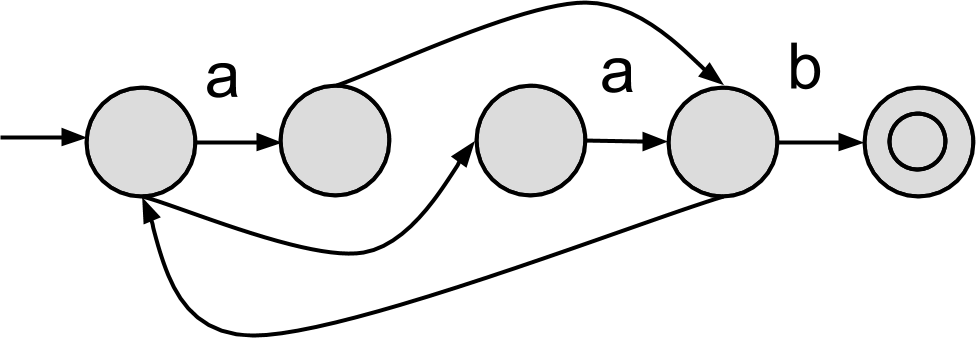
\includegraphics[scale=0.3]{figures/exemplo_automato.png}
  \caption{Exemplo de autômato para expressão regular $(a|a)+b$}
  \label{fig:exemplo_automato}
\end{figure}

Desde então, conforme as implementações foram evoluindo, muitas funcionalidades foram adicionadas à linguagem de descrição de expressões regulares que as afastaram da teoria original. Enquanto originalmente descreviam linguagens estritamente regulares, a implementação mais difundida atualmente (\emph{PCRE}) é capaz não só de reconhecer qualquer linguagem livre de contexto, como também algumas sensíveis a contexto. \cite{bib:Nikita12}

Uma das consequências mais notáveis desta evolução não planejada é que o reconhecimento de strings da linguagem, um problema com solução linear originalmente, ganhou soluções exponenciais em um grande número de implementações modernas, que inclui muitas das mais usadas. Talvez a funcionalidade mais perigosa neste sentido sejam as backreferences, que não só impedem soluções polinomiais como tornam o problema de reconhecimento NP-completo. Entretanto, mesmo nas expressões que poderiam ser reconhecidas estritamente com autômatos finitos, certas particularidades de implementação as tornam potencialmente exponenciais, no pior caso \cite{bib:Cox07}.

A figura \ref{fig:benchmark1} mostra o crescimento no tempo de execução entre a implementação da biblioteca padrão da linguagem Python e a implementação proposta neste projeto, usando o método de Thompson. 

\begin{figure}[ht]
  \centering
  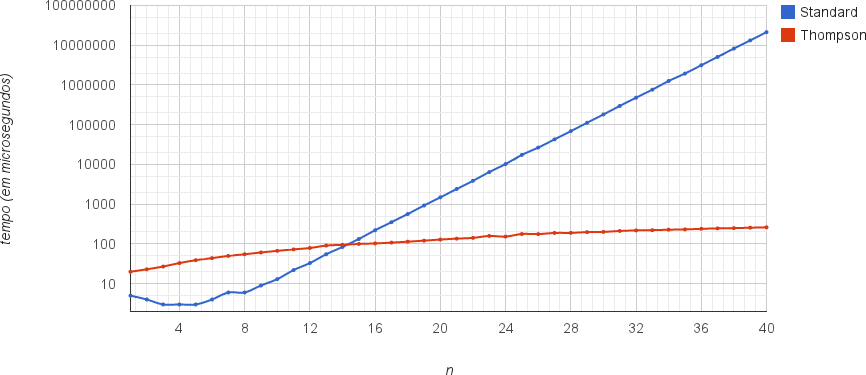
\includegraphics[scale=0.5]{figures/benchmark1.png}
  \caption{Avaliação da string $a^n$ contra a expressão $(a|a)+b$ (em escala logarítmica)}
  \label{fig:benchmark1}
\end{figure}

Essas implementações tornam o uso de expressões regulares potencialmente inseguro em situações ora triviais. Um usuário mal intencionado pode ser capaz de forçar a execução de uma expressão com caráter exponencial para efetuar um ataque de negação de serviço em um servidor web, por exemplo. 

Muitas vezes a prevenção para esse tipo de ataque pode não ser trivial, e.g. em Java, onde métodos comumente usados contra a entrada do usuário, como \emph{replaceAll} e \emph{split}, da classe \emph{String} são implementados usado expressões regulares vulneráveis a esse tipo de ataque.

Mesmo em casos onde o usuário mal intencionado não tem acesso a escrever expressões regulares, um erro de programação pode deixar o sistema vulnerável a negação de serviço. Este problema torna-se especialmente notável pelo frequente compartilhamento em repositórios online, que contém muitas expressões vulneráveis \cite{bib:Kirrage13,bib:Weidman10}. 

%~~~~~~~~~~~~~~~~~~~~~~~~~~~~~~~~~~~~~~~~~~~~~~~~~~~~~~~~~~~~~~~~~~~~~~~
\section{Objetivo}
%~~~~~~~~~~~~~~~~~~~~~~~~~~~~~~~~~~~~~~~~~~~~~~~~~~~~~~~~~~~~~~~~~~~~~~~

Este projeto tem dois objetivos principais. O primeiro é demonstrar através de testes pontuais e benchmarks os problemas fundamentais nas implementações de expressões regulares em diversas linguagens modernas, provando inclusive a NP-completude do problema de reconhecimento de strings nas linguagens que definem. O segundo objetivo é propor uma implementação didática e minimalista das expressões regulares propostas por Kleene, utilizando o método descrito por Thompson para construção e simulação do autômato. 

A implementação irá deixar de fora certas funcionalidades comuns nos \emph{sabores} mais modernos de expressão regular. Algumas destas funcionalidades podem ser implementadas sem sacrificar eficiência de execução. Outras, introduzem certa complexidade, porém mantendo a execução do algoritmo polinomial. O restante, entretanto, não é possível implementar sem tornar o algoritmo exponencial no pior caso. Todas as funcionalidades intencionalmente excluídas serão listadas e propostas de soluções serão apresentadas quando cabível.

Deseja-se mostrar com esse projeto que o problema de reconhecimento de expressões regulares pode ser resolvido de maneira eficiente, mesmo com as implementações mais simples, desde que seja observada a base teórica que as deu origem.

%~~~~~~~~~~~~~~~~~~~~~~~~~~~~~~~~~~~~~~~~~~~~~~~~~~~~~~~~~~~~~~~~~~~~~~~
\section{Estrutura}
%~~~~~~~~~~~~~~~~~~~~~~~~~~~~~~~~~~~~~~~~~~~~~~~~~~~~~~~~~~~~~~~~~~~~~~~

O projeto está divido em cinco capítulos. O capítulo 2 trata da base teórica por trás das expressões regulares, contando sua história, passando pelo método de construção do autômato de Thompson, e exibindo um algoritmo trivial (porém ineficiente) para sua solução.

O capítulo 3 descreve a implementação sugerida por este trabalho, discutindo certos aspectos específicos desta implementação que não tenham sido abordados na parte de teoria. 

O capítulo 4 aborda as diferenças entre as implementações modernas e a implementação proposta neste trabalho. Começa descrevendo o poder das implementações modernas de expressão regular, mostrando recursos avançados, como \emph{zero-width assertions} e \emph{backreferences}. Prova a NP-completude do \emph{match} nestas implementações. Mostra também exemplos de expressões que reconhecem gramáticas não-regulares, exibindo o distanciamento entre estas e a teoria original. Por fim, é mostrado um benchmark comparando as diversas implementações, que evidenciam uma diferença fundamental na forma como o problema é abordado em cada uma delas.

O capítulo 5 expõe as conclusões e contribuições deste trabalho, bem como as dificuldades encontradas durante o projeto. Também serão listadas e descritas as funcionalidades não implementadas, possivelmente sugerindo formas eficientes de implementá-las, ou mesmo formas diferentes de simular o autômato que melhorem a eficiência geral da execução.

%======================================================================================
\chapter{Fundamentação Teórica}
%======================================================================================

Neste capítulo será introduzida um pouco da base teórica que guiou a implementação deste projeto.

%~~~~~~~~~~~~~~~~~~~~~~~~~~~~~~~~~~~~~~~~~~~~~~~~~~~~~~~~~~~~~~~~~~~~~~~
\section{Linguagens Formais}
%~~~~~~~~~~~~~~~~~~~~~~~~~~~~~~~~~~~~~~~~~~~~~~~~~~~~~~~~~~~~~~~~~~~~~~~

Linguagens formais é um tema que mistura elementos da ciência da computação, matemática e linguística. Seu papel na computação é fundamental pela relação de seus problemas com os descritos pela teoria da computação.

Uma \emph{linguagem formal} é um conjunto -- potencialmente infinito -- de \emph{palavras}, que por sua vez são combinações de elementos de um conjunto finito de símbolos chamado \emph{alfabeto}.

\subsection{Palavra}

Palavras são combinações entre os elementos de um alfabeto. Por exemplo, com um alfabeto $\Sigma = \{0, 1\}$, é possível formar palavras que representam números binários.

Uma palavra é representada pelos símbolos que a compõem. Logo, 01101 é uma palavra formada pelos símbolos do alfabeto descrito anteriormente. Uma palavra especial, denotada $\epsilon$ (às vezes $\lambda$) representa uma palavra vazia.

Dado um alfabeto com $k$ símbolos, é possível formar até $k^n$ palavras de tamanho $n$. Logo, existem

\begin{equation*}
	\mathlarger \sum^{n}_{i=0} k^i = \frac{k^{n+1}-1}{k-1}
\end{equation*}

palavras de até $n$ caracteres num alfabeto com $k$ símbolos.

O conjunto formado por todas as palavras de um alfabeto é infinito, porém enumerável. Uma possível estratégia é numerá-los primeiro por seu tamanho, então por sua ordem lexicográfica.

A operação básica entre palavras é a \emph{concatenação}. Por exemplo, 

\begin{alignat*}{3}
w_1 = aaa &\wedge w_2=bbb  &\rightarrow w_1w_2 &= aaabbb \\
w_1 = aaa &\wedge w_2=\epsilon  &\rightarrow w_1w_2 &= aaa \\
w_1 = \epsilon &\wedge w_2=bbb  &\rightarrow w_1w_2 &= bbb \\
\end{alignat*}

Concatenação é associativa, então 

\begin{equation*}
(w_1w_2)w_3 = w_1(w_2w_3),
\end{equation*}

porém não comutativa, logo

\begin{equation*}
w_1w_2 \neq w_2w_1.
\end{equation*}

\subsection{Linguagem}

Linguagens são conjuntos de palavras sobre algum alfabeto. A mesma notação de conjuntos é utilizada para elas. Por exemplo, $A \cup B$ representa a linguagem formada pela união de todas as palavras de A e B, assim como $w \in A$ é uma proposição afirma que a palavra $w$ está presente na linguagem A.

É possível concatenar linguagens. Dadas linguagens $L_1$ e $L_2$,

\begin{equation*}
	L_1L_2 = \{w_1w_2 \mid w_1 \in L_1, w_2 \in L_2\}
\end{equation*}

E.g.: se $A = \{a, aa\}$ e $B = \{b, bb\}$, então $AB = \{ab, aab, abb, aabb\}$.


Com base na concatenação, uma operação importante em linguagens é o fecho Kleene (ou fecho de concatenação, $L^*$), que pode ser definido recursivamente como:

\begin{equation*}
	L^0 = \{\epsilon\}
\end{equation*}
\begin{equation*}
	L^i = L^{i-1}L
\end{equation*}
\begin{equation*}
	L^* = \bigcup_{i \in \mathbb{N}} L^i
\end{equation*}

E.g.: se $A = \{a, aa\}$, então $A^* = \{\epsilon, a, aa, aaa, \ldots\}$.

Existem duas formas principais para se definir linguagens formais. \emph{Gramáticas gerativas}, que geram elementos da linguagem a partir de sistemas de reescrita; e \emph{Autômatos}, que reconhecem elementos da linguagem. 

Além destas, existem diversas outras formas de definir linguagens. As próprias expressões regulares denotam linguagens formais. Outra forma bastante é comum é através da sintaxe de geração de conjuntos, e.g. $L=\{a^n \mid n \in \mathbb{N}\}$.

%~~~~~~~~~~~~~~~~~~~~~~~~~~~~~~~~~~~~~~~~~~~~~~~~~~~~~~~~~~~~~~~~~~~~~~~
\section{Gramáticas Gerativas}
%~~~~~~~~~~~~~~~~~~~~~~~~~~~~~~~~~~~~~~~~~~~~~~~~~~~~~~~~~~~~~~~~~~~~~~~

Uma das formas de representar linguagens formais é através de gramáticas gerativas. O termo ``gramática formal'' é comumente utilizado para referir-se a elas. No entanto, existem outras formas de representar gramáticas formais além deste.

Gramáticas gerativas são sistemas de reescrita, i.e. a partir de um símbolo inicial, é possível usar as regras de reescrita para produzir todas as palavras de uma linguagem. Esta operação é, de certa forma, o problema dual de reconhecer uma palavra como parte da linguagem através de um autômato \cite{bib:Ruohonen09}.

Uma gramática gerativa é formada por uma tupla $G = (N, \Sigma, P, S)$. Onde:

\begin{lcircp}
    \item N é o conjunto de símbolos não terminais. Eles não fazem parte da linguagem original, então precisam ser sempre substituídos para alcançar um símbolo válido na linguagem.
    \item $\Sigma$ é o conjunto de símbolos terminais da linguagem. Também conhecido como alfabeto.
    \item P é o conjunto de regras de produção, geralmente na forma $\alpha \rightarrow \beta \mid \alpha, \beta \in N \cup \Sigma$.
    \item S é o símbolo inicial do sistema de reescrita. $S \in N$.
\end{lcircp}

Um exemplo de gramática é a que define expressões da forma $a^nb^n, n>0$:

\begin{equation*}
	G = ({\{S\}, \{a,b\}, P, S})
\end{equation*}

Onde P é definido por:

\begin{equation*}
	S \rightarrow aSb
\end{equation*}
\begin{equation*}
	S \rightarrow ab
\end{equation*}

Iniciando do símbolo S, é possível começar com a regra $ab$ ou $aSb$. A primeira já forma uma palavra na linguagem que queremos descrever ($ab$), a segunda possui um símbolo não terminal. A partir dele é possível gerar as palavras na linguagem: $aabb$, $aaabbb$, etc...

Perceba que na gramática todas as regras do lado esquerdo possuem apenas um símbolo não terminal. Se fôssemos escrever uma gramática para expressões na forma $a^nb^nc^n$, precisaríamos de uma gramática mais rebuscada:

\begin{equation*}
	G = (\{S, T\}, \{a,b,c\}, P, S)
\end{equation*}

Onde P é definido por:

\begin{equation*}
	S \rightarrow aTSc
\end{equation*}
\begin{equation*}
	S \rightarrow abc
\end{equation*}
\begin{equation*}
	Ta \rightarrow aT
\end{equation*}
\begin{equation*}
	Tb \rightarrow bb
\end{equation*}

O fato desta gramática definir sequências de símbolos à esquerda com mais de um símbolo a torna especial. Segundo a hiearquia de Chomsky, a primeira gramática é livre de contexto, enquanto a segunda é sensível a contexto.

%~~~~~~~~~~~~~~~~~~~~~~~~~~~~~~~~~~~~~~~~~~~~~~~~~~~~~~~~~~~~~~~~~~~~~~~
\section{Hierarquia de Chomsky}
%~~~~~~~~~~~~~~~~~~~~~~~~~~~~~~~~~~~~~~~~~~~~~~~~~~~~~~~~~~~~~~~~~~~~~~~

Segundo Noam Chomsky \cite{bib:Chomsky57}, uma gramática formal pode ser classificada em um de quatro tipos baseados em sua capacidade expressiva:

\begin{lcircp}
    \item {\bf Tipo 0}: gramáticas recursivamente enumeráveis (ou irrestritas)
    \item {\bf Tipo 1}: gramáticas sensíveis a contexto
    \item {\bf Tipo 2}: gramáticas livres de contexto
    \item {\bf Tipo 3}: gramáticas regulares
\end{lcircp}

Cada conjunto é propriamente incluso no seu conjunto superior na hierarquia, como pode ser visto na figura~\ref{fig:chomsky}.

\begin{figure}[ht]
  \centering
  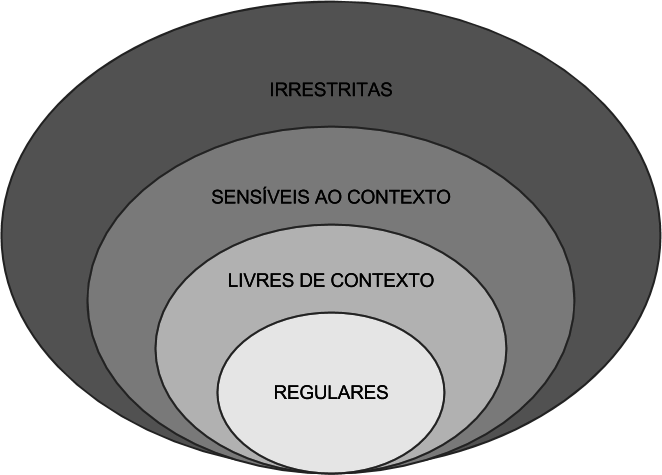
\includegraphics[scale=0.5]{figures/chomsky.png}
  \caption{Representação da inclusão de conjuntos na hiearquia de Chomsky}
  \label{fig:chomsky}
\end{figure}

\subsection{Gramáticas Regulares}

Gramáticas regulares são aquelas cujas regras de formação são na forma $S \rightarrow a$ ou $S \rightarrow aT$, onde \emph{S} e \emph{T} são não-terminais e \emph{a} é um terminal na linguagem. Estas linguagens são equivalentes em poder de expressão a \emph{autômatos finitos}. 

Opcionalmente a regra $S \rightarrow aT$ pode ser substituída por $S \rightarrow Ta$, mas nunca as duas podem ocorrer na mesma gramática. Se a primeira ocorre, a gramática é conhecida como \emph{regular à direita}. Caso contrário, é \emph{regular à esquerda}.

Alguns autores também incluem regras do tipo $S \rightarrow \epsilon$, desde que S não apareça do lado direito de nenhuma regra.

Exemplos de linguagens regulares incluem: endereços de email, repetição de caracteres ($a^n$), repetição independente de dois caracteres ($a^nb^m$).

\subsection{Gramáticas Livres de Contexto}

Gramáticas livres de contexto são aquelas onde todas as regras de formação são do tipo $S \rightarrow \gamma$, onde \emph{S} é um não-terminal e $\gamma$ é uma sequência composta por terminais e não-terminais. 

Isto na prática significa que a substituição de um não-terminal é sempre feita independente do contexto onde é encontrado. Linguagens deste tipo são equivalentes em poder expressivo a \emph{autômatos de pilha}. Elas compõem a base teórica para a maioria das linguagens de programação. 

Entre alguns exemplos clássicos de linguagens livres de contexto figuram: parênteses aninhados, repetição condicionada de dois caracteres ($a^nb^n$), expressões aritméticas.

\subsection{Gramáticas Sensíveis a Contexto}
Gramáticas sensíveis a contexto são aquelas onde todas as regras de formação são do tipo $\alpha S\beta\rightarrow \alpha\gamma\beta$, onde $\alpha$, $\gamma$ e $\beta$ são sequências compostas por terminais e não-terminais. Elas diferem das gramáticas livres de contexto por definir -- exatamente -- contexto para que um não-terminal S seja substituído por uma sequência $\gamma$. 

Apesar de terem um escopo bem mais amplo, gramáticas deste tipo ainda são passíveis de ser computadas usando um \emph{autômato linearmente limitado}. 

Exemplos de liguagens sensíveis a contexto: \emph{squares} (\emph{DogDog, CatCat, WikiWiki...}), \emph{matching triplets} ($a^nb^nc^n$).

\subsection{Gramáticas Recursivamente Enumeráveis}

Gramáticas recursivamente enumeráveis não definem restrições para as regras de produção. Portanto, qualquer sequência de terminais e não-terminais $\alpha$ pode ser substituída por outra $\beta$. Gramáticas assim são reconhecíveis por uma \emph{máquina de Turing}. 

Diferente dos tipos anteriores, quando apresentada a uma sequência que não faça parte da linguagem, não há garantia de parada da máquina, definindo o que é chamado de \emph{conjunto semi-decidível}.

Um dos exemplos mais notáveis de linguagens recursivamente enumeráveis que não são sensíveis a contexto é a sintaxe de templates do C++ \cite{bib:Veldhuizen03}.

\subsection{Tabela de Referência}

É possível resumir os tipos de gramáticas da hierarquia de Chomsky numa tabela de referência quanto à máquina que a processa e os tipos de regras que aceita.

\begin{center}
	\begin{tabular}{ c | c | c | c }
		 & {\bf Linguagem} & {\bf Máquina} & {\bf Regras} \\
		\hline 
		0 & Recursivamente enumerável & Máquina de Turing 			 & 
			$\alpha \rightarrow \beta$ \\ 
		1 & Sensível a contexto 		& Autômato limitado linearmente & 
			$\alpha S\beta\rightarrow \alpha\gamma\beta$\\ 
		2 & Livre de contexto 			& Autômato de pilha 			 & 
			$S \rightarrow \gamma$\\ 
		3 & Regular 					& Autômato finito 				 &
			$S \rightarrow aT$ ou $S \rightarrow a$\\ 
	\end{tabular}
\end{center}

%~~~~~~~~~~~~~~~~~~~~~~~~~~~~~~~~~~~~~~~~~~~~~~~~~~~~~~~~~~~~~~~~~~~~~~~
\section{Expressões Regulares}
%~~~~~~~~~~~~~~~~~~~~~~~~~~~~~~~~~~~~~~~~~~~~~~~~~~~~~~~~~~~~~~~~~~~~~~~

Expressões regulares são sequências de caracteres que definem linguagens regulares. Estas sequências obedecem a algumas regras de criação. Alguns caracteres são interpretados literalmente, enquanto outros são considerados metacaracteres que controlam como os trechos da expressão se relacionam.

Por definição:

\begin{lcircp}
    \item Sequências vazias são expressões regulares.
    \item Caracteres unitários são expressões regulares. E.g. \emph{a}.
    \item Expressões regulares podem ser concatenadas para formar novas expressões. E.g. se $e_1$ reconhece \emph{a} e $e_2$ reconhece \emph{b}, então $e_1e_2$ reconhece \emph{ab}.
    \item Expressões regulares podem ser alternadas para formar novas expressões. E.g. se $e_1$ reconhece \emph{a} e $e_2$ reconhece \emph{b}, então $e_1|e_2$ reconhece \emph{a} e \emph{b}.
    \item Pode-se aplicar o fecho Kleene para formar novas expressões. E.g. se $e_1$ reconhece \emph{a}, então $e_1*$ reconhece \emph{a}, \emph{aa}, \emph{aaa}... etc., bem como string vazia.
\end{lcircp}

Perceba que é possível definir outros operadores comuns, como $?$ e $+$. Mas é possível fazê-lo a partir das operações descritas acima. O operador $e_1?$ pode ser definido como a alternância entre $e_1$ e uma string vazia. O operarador $e_1+$ pode ser definido como $e_1e_1*$.

Outros operadores sobre caracteres como o $.$ (qualquer caractere) e as classes de caractere (e.g. $[a-zA-Z]$) são trivialmente implementados usando alternação de expressões.

A precedência natural dos operadores, da mais fraca para a mais forte, é: alternância, concatenação, repetição. Assim, uma expressão como $ab|cd*$ é interpretada como exibido na figura~\ref{fig:abcd_parse_tree}.

\begin{figure}[ht]
  \centering
  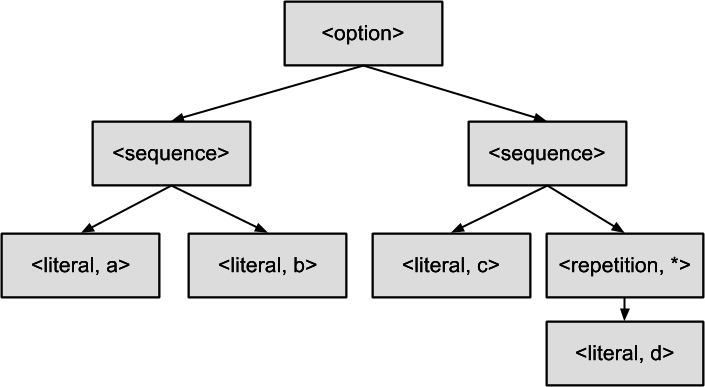
\includegraphics[scale=0.4]{figures/abcd_parse_tree.png}
  \caption{Árvore de avaliação para expressão $ab|cd*$}
  \label{fig:abcd_parse_tree}
\end{figure}

É possível agrupar sub-expressões utilizando parênteses, tal qual é feito com expressões aritméticas. Assim $a(b|c)d*$ tem um sentido completamente diferente de $ab|cd*$.

Estas operações, apesar de bastante incompletas, definem inequivocamente expressões regulares. É possível representar qualquer linguagem regular utilizando apenas estes operadores. Mais importante: é teoricamente possível reconhecer qualquer símbolo nesta linguagem com apenas uma passagem pela entrada (sem \emph{backtracking}). 

Representando apenas linguagens regulares, as expressões regulares representam um paradoxo sobre si mesmas: elas não são capazes de representar nem a própria linguagem que as define. O grande culpado disso é a presença dos parênteses agrupadores, tornando esta gramática propriamente pertencente ao conjunto das gramáticas livres de contexto.

Novas implementações de expressões regulares adicionaram novos operadores que tornam a sintaxe mais concisa. Porém, essas adições normalmente não alteram o poder expressivo das regexes. No entanto, existem adições que adicionam poder expressivo, como é o caso das \emph{backreferences}, que permitem o reconhecimento de algumas linguagens não-regulares. \emph{Backreferences} consiste em referências \emph{submatches} reconhecias anteriormente.

Por exemplo, uma linguagem composta por palavras repetidas, como \emph{DogDog} ou \emph{CatCat}. É possível definir uma expressão regular $/(.*)\backslash 1/$ que reconhece esta linguagem. o $\backslash 1$ instrui ao motor de reconhecimento a esperar uma nova palavra exatamente igual à obtido pelo reconhecimento do primeiro grupo $(.*)$.

Esta linguagem não apenas cai fora do conjunto das linguagens regulares, como também não é uma linguagem livre de contexto.

Tal poder expressivo tem seu preço. Match de backreferences é um problema NP-completo, logo, os melhores algoritmos conhecidos ainda tem pior caso exponencial. É possível, porém, escrever algoritmos polinomiais para expressões que não fazem uso de backreferences. No entanto, pela diferente natureza dos dois tipos de algoritmos, normalmente as linguagens implementam apenas um deles, fazendo com que algumas expressões que originalmente poderiam ser avaliadas em tempo polinomial serem penalizadas sem necessidade.

%~~~~~~~~~~~~~~~~~~~~~~~~~~~~~~~~~~~~~~~~~~~~~~~~~~~~~~~~~~~~~~~~~~~~~~~
\section{Autômatos Finitos}
%~~~~~~~~~~~~~~~~~~~~~~~~~~~~~~~~~~~~~~~~~~~~~~~~~~~~~~~~~~~~~~~~~~~~~~~

Autômatos finitos representam um modelo matemático de computação. Eles representam máquinas abstratas que podem se encontram em apenas um de um número finito de estados. Autômatos não possuem memória. Mas apenas estritamente falando, pois o estado atual do autômato representa sua memória. Um autômato muda de estado como reação a um estímulo externo. Formalmente, autômatos finitos são uma tupla $M = (Q, \Sigma, q_0, \delta, A)$, onde:

\begin{lcircp}
    \item Q é o conjunto de estados do autômato. Sempre finito.
    \item $\Sigma$ é o alfabeto aceito pelo autômato.
    \item $q_0$ é o estado inicial do autômato. $q_0 \in Q$.
    \item $\delta$ é a função de transição, que mapeia cada $(q_i, a) \in Q \times \Sigma$ a um subconjunto de Q. Se esse subconjunto tem apenas zero ou um elementos, o autômato é \emph{deterministico}, caso contrário, ele é \emph{não-determinístico}.
    \item A é o conjunto de estados de aceite. $A \subseteq Q$.
\end{lcircp}

Por exemplo:

\begin{figure}[ht]
  \centering
  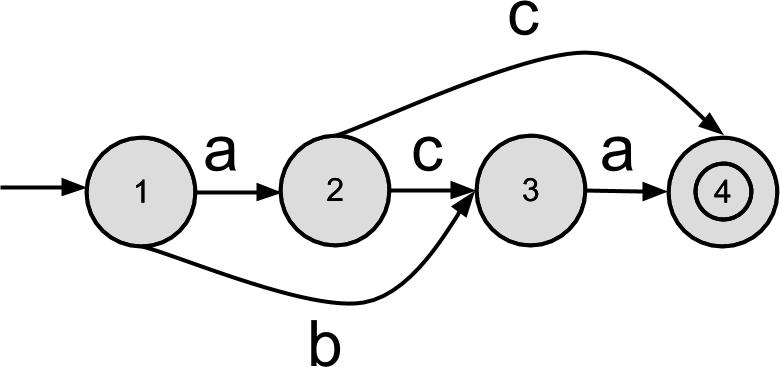
\includegraphics[scale=0.3]{figures/exemplo_automato_numerado.png}
  \caption{Diagrama de estados de um autômato não-determinístico}
  \label{fig:exemplo_automato_numerado}
\end{figure}

O autômato na figura~\ref{fig:exemplo_automato_numerado} pode ser descrito por $M=(\{1,2,3,4\}, \{a,b,c\}, 1, \delta, \{4\})$, onde $\delta$ é definida pela tabela de transições:

\begin{center}
	\begin{tabular}{ c || c | c | c }
		{\bf $\delta$} & {\bf a} & {\bf b} & {\bf c} \\
		\hline 
		\hline 
		1 & 2 & 3 &  \\ 
		\hline 
		2 &   &   & 2, 4 \\ 
		\hline 
		3 & 4 &   &  \\ 
		\hline 
		4 &   &   &  \\ 
	\end{tabular}
\end{center}

Este autômato é \emph{não determinístico}, pois um mesmo input (c) pode gerar múltiplas transições no estado 2. 

Outra forma de representar autômatos não determínisticos é introduzindo a entrada $\epsilon$, como pode ser visto na figura~\ref{fig:exemplo_automato_epsilon}. Perceba que este autômato \emph{não é equivalente} ao definido anteriormente. Ele aceita uma entrada $b$ que o primeiro não aceita.

\begin{figure}[ht]
  \centering
  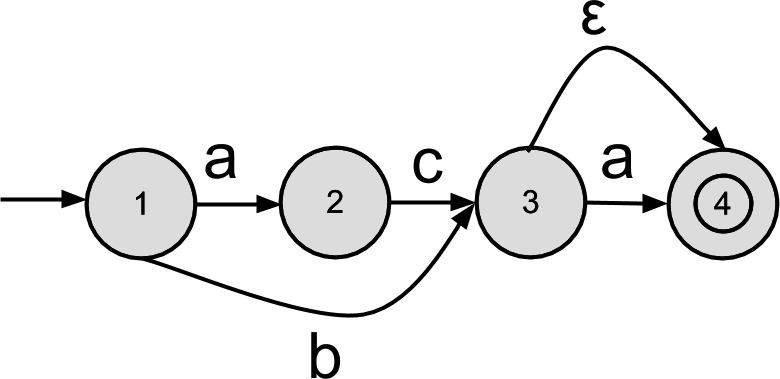
\includegraphics[scale=0.3]{figures/exemplo_automato_epsilon.png}
  \caption{Diagrama de estados de um autômato não-determinístico com entrada $\epsilon$}
  \label{fig:exemplo_automato_epsilon}
\end{figure}


Autômatos podem ser utilizados para reconhecer linguagens regulares. É possível construir um autômato que, dada uma linguagem, termina em estados de aceite somente se a palavra fizer parte da linguagem representada.

O autômato descrito na figura~\ref{fig:exemplo_automato_epsilon}, por exemplo, reconhece uma linguagem finita definida por $L = \{ac, aca, b, ba\}$. A linguagem que um autômato finito reconhece é \emph{sempre regular}. E \emph{toda linguagem regular} pode ser reconhecida com autômatos finitos \cite{bib:Kleene56}.

%~~~~~~~~~~~~~~~~~~~~~~~~~~~~~~~~~~~~~~~~~~~~~~~~~~~~~~~~~~~~~~~~~~~~~~~
\section{Método de Construção de Thompson}
%~~~~~~~~~~~~~~~~~~~~~~~~~~~~~~~~~~~~~~~~~~~~~~~~~~~~~~~~~~~~~~~~~~~~~~~

Pela equivalência entre linguagens regulares e autômatos finitos. É útil poder converter entre um e outro pela facilidade de lidar com cada um deles em situações específicas. Ken Thompson \cite{bib:Thompson68} descreveu um método para construir autômatos a partir de expressões regulares.

Na época em que foi escrito, o artigo descrevia como gerar código de máquina para um IBM 7094. Isto era necessário por restrições de hardware da época. Hoje não é mais estritamente necessário. Este trabalho irá se limitar a descrever como construir o autômato a partir da expressão regular.

O método consite em construir o autômato recursivamente através da análise da árvore sintática da expressão, procedimento que precisa ser efetuado antes do começo da construção do autômato. No artigo original de Thompson, este passo era feito construindo a expressão em notação \emph{infixa}. Entretanto, para permitir extensibilidade do formato da expressão, iremos definir completamente a gramática da expressão regular que aceitaremos.

\subsection{Analise sintática}

O primeiro passo para a construção do autômato é analisar sintaticamente a expressão, construindo a árvore sintática. 

Podemos definir uma EBNF simples que representa a linguagem formada pelas expressões regulares.

\begin{verbatim}
<option>     ::= <sequence> { "|" <sequence> }*
<sequence>   ::= <repetition> { <repetition> }*
<repetition> ::= <primary> { "*" | "?" | "+" }*
<primary>    ::= "." | <literal> | "(" <option> ")"
\end{verbatim}

Assim, podemos fazer parse da expressão facilmente. A expressão $(a|a)+b$, por exemplo, seria avaliada como a árvore descrita na figura~\ref{fig:aab_parse_tree}.

\begin{figure}[ht]
  \centering
  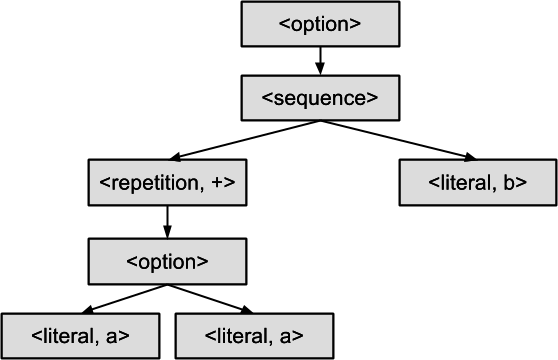
\includegraphics[scale=0.5]{figures/aab_parse_tree.png}
  \caption{Árvore de avaliação para expressão $(a|a)+b$}
  \label{fig:aab_parse_tree}
\end{figure}

Utilizando a EBNF, esta árvore pode ser produzida por diversos tipos de ferramentas presentes em várias linguagens. Exemplos notáveis incluem o YACC (\emph{Yet Another Compiler Compiler}) e o JAVACC (\emph{Java Compiler Compiler}).

Com esta árvore de avaliação é possível fazer a conversão para o autômato de forma bastante trivial, como será discutido nas próximas seções.

\subsection{Notação}
\label{sec:Notacao}

Iremos assumir uma notação diferente para representação do autômato, que irá facilitar a construção. Para fins de praticidade, todo estado $q_i \in Q$ será de um entre três tipos possíveis:

\begin{lcircp}
    \item Um estado de \emph{consumo}, que possui exatamente uma transição possível dada por um caractere $a \in \Sigma$.
    \item Um estado de \emph{decisão}, que possui uma ou duas transições $\epsilon$ para estados distintos.
    \item Um estado de \emph{aceite}, que não possui qualquer transição.
\end{lcircp}

A figura~\ref{fig:nova_notacao} mostra como podem ser representados os estados desta nova notação no diagrama de estados.

\begin{figure}[ht]
  \centering
  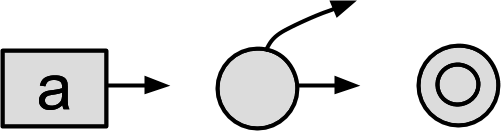
\includegraphics[scale=0.5]{figures/nova_notacao.png}
  \caption{Representação de estados na nova notação}
  \label{fig:nova_notacao}
\end{figure}

Esta representação facilita a visualização por omitir as transições $\epsilon$ e ressaltar a diferença entre os estados de consumo e os estados de decisão. Um exemplo de conversão para a nova notação pode ser visto na figura~\ref{fig:exemplo_nova_notacao}.

\begin{figure}[ht]
  \centering
  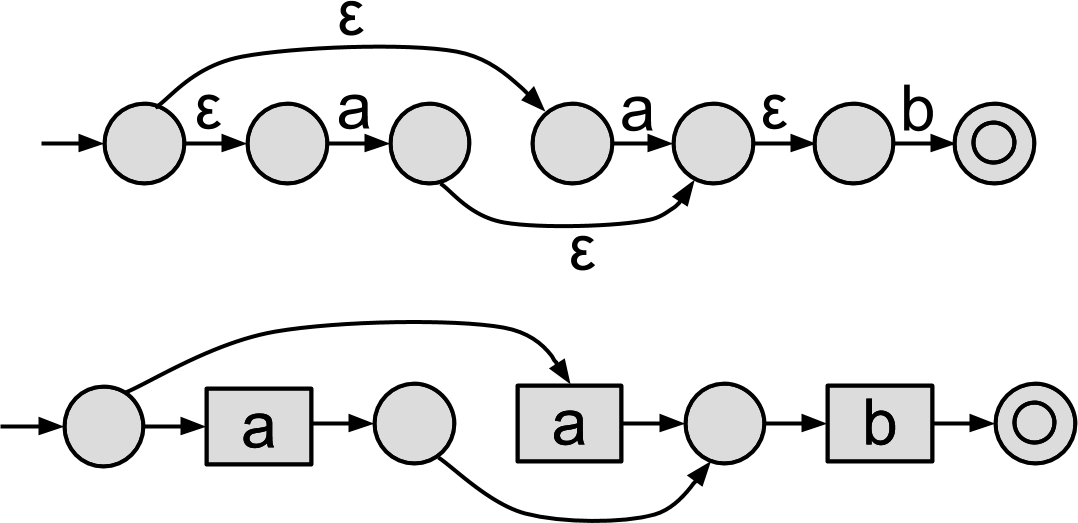
\includegraphics[scale=0.25]{figures/exemplo_nova_notacao.png}
  \caption{Mesmo autômato representado com as duas notações}
  \label{fig:exemplo_nova_notacao}
\end{figure}

\subsection{Construção}

A construção do autômato se dá pela conversão recursiva de cada um dos nós na árvore por uma construção de autômato predeterminada. Cada uma destas construções tem apenas um estado de entrada e todas as transições que não apontem para um nó dentro da própria construção, apontam para um único nó de saída.

Em uma implementação otimizada, este passo pode ser substituído por geração de código de máquina (como no artigo original). Entretanto, para fins didáticos, abordaremos algumas representações úteis do autômato gerado.

A tabela a seguir mostra a conversão para cada tipo de nó. Para fins de notação, as letras maiúsculas representam autômatos complexos produzidos em passos anteriores, mas que seguem a mesma regra definida no parágrafo anterior.

\begin{center}
	\begin{tabular}{ c | c | c }
		{\bf Tipo} & {\bf Expressão} & {\bf Construção} \\
		\hline
		\hline
		Literal & $a$ & 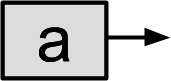
\includegraphics[scale=0.25]{figures/thompson_literal.png} \\ 
		\hline
		Sequência & $ST$ & 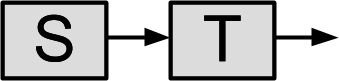
\includegraphics[scale=0.25]{figures/thompson_sequence.png} \\ 
		\hline
		Opção & $S|T$ & 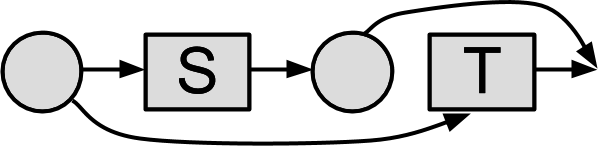
\includegraphics[scale=0.25]{figures/thompson_option.png} \\ 
		\hline
		Kleene+ & $S+$ & 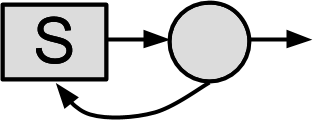
\includegraphics[scale=0.25]{figures/thompson_plus.png} \\ 
		\hline
		Opcional & $S?$ & 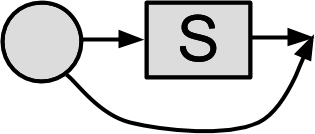
\includegraphics[scale=0.25]{figures/thompson_question.png} \\ 
		\hline
		Kleene* & $S*$ & 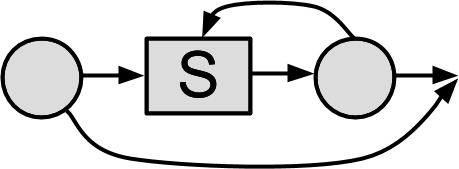
\includegraphics[scale=0.25]{figures/thompson_kleene.png} \\ 
		\hline
	\end{tabular}
\end{center}

Para converter um autômato usando estas regras, basta percorrer a árvore de avaliação de baixo para cima, inicialmente transformando todos os literais e recursivamente usando-os como insumo para os nós superiores. A figura~\ref{fig:exemplo_automato_completo} mostra um exemplo de conversão utilizando a expressão $(a|a)+b$.

\begin{figure}[ht]
  \centering
  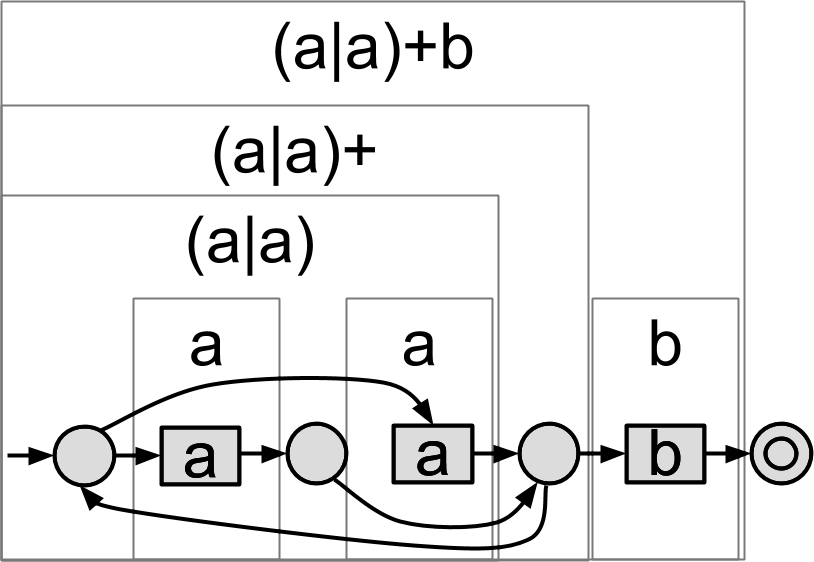
\includegraphics[scale=0.33]{figures/exemplo_automato_completo.png}
  \caption{Exemplo completo de autômato para a expressão $(a|a)+b$}
  \label{fig:exemplo_automato_completo}
\end{figure}

Uma das vantagens desta forma de construir é que ela pode ser escrita como uma sequência de instruções para serem interpretadas por uma máquina virtual. Cada um dos três tipos de estados definidos pela notação na seção anterior podem ser substituídos por uma entre três instruções. Estados de consumo como instruções \emph{CONSUME}, estados de decisão como instruções \emph{JUMP} e estados de aceite como instruções \emph{MATCH}.

Por exemplo, o autômato representado pela figura~\ref{fig:exemplo_automato_completo} pode ser reescrito como as instruções:

\nopagebreak 
\begin{verbatim}
0000: JUMP (1, 3)
0001: CONSUME a
0002: JUMP (2,)
0003: CONSUME a
0004: JUMP (1, -4)
0005: CONSUME b
0006: MATCH!
\end{verbatim}

As instruções \emph{JUMP} são os que representam o não-determinismo destes autômatos, pois ao serem executadas, podem mudar para qualquer um dos rótulos para os quais apontam. Existem diversas formas de simular a execução desses programas não-determinísticos usando uma máquina de Turing determínistica. E é exatamente neste ponto onde a maior parte das implementações torna-se exponencial desnecessariamente.

%~~~~~~~~~~~~~~~~~~~~~~~~~~~~~~~~~~~~~~~~~~~~~~~~~~~~~~~~~~~~~~~~~~~~~~~
\section{Simulação do Autômato}
%~~~~~~~~~~~~~~~~~~~~~~~~~~~~~~~~~~~~~~~~~~~~~~~~~~~~~~~~~~~~~~~~~~~~~~~

Simular a execução de um autômato não-determinístico utilizando uma máquina determinística é um problema por si só complicado. Existem potencialmente exponenciais caminhos possíveis num autômato não-determinístico \cite{bib:Rabin59}.

Dentre as opções para simulação da execução do autômato, estão:

\begin{lcircp}
    \item \emph{Backtracking}: tentar todos os caminhos possíveis, voltando para a última escolha feita em caso de falha.
    \item \emph{Backtracking com memoização}.
    \item \emph{Conversão para DFA}: converter para um autômato determinístico antes de executar.
    \item \emph{Simulação paralela}: simular a execução de todos os estados simultaneamente.
	\item \emph{Conversão preguiçosa para DFA}: semelhante a execução paralela, mas construindo um cache dos estados alcançados
\end{lcircp}

Cada uma destas opções tem caracteristicas próprias. Suas vantagens e desvantagens serão discutidas separadamente.

\subsection{Backtracking}

Backtracking é talvez a forma mais trivial de implementar a simulação de autômatos não determinísticos. Consiste basicamente em ao ser apresentado a uma escolha, decidir por uma delas, mas manter uma pilha de escolhas feitas para retroceder e escolher novamente caso não tenha sucesso.

\emph{Vantagem}: Este método é o mais fácil de implementar, pois como a chamada de subrotinas na maior parte das linguagens já implementa uma pilha, uma simples recursão é o suficiente para implementar esta técnica.

\emph{Desvantagem}: Pela natureza do autômato, cada escolha pode gerar vários fluxos independentes, então uma sequência de n escolhas (assumindo que sejam binárias) pode gerar até $2^n$ fluxos diferentes. Além disso, esta técnica requer múltiplas passagens pela mesma string, o que é trivial se ela estiver em memória, mas complicado se estiver vindo de um fluxo de rede ou pipes do sistema. E por fim, a pilha reservada para chamadas de métodos é compartilhada com outros recursos e limitada em diversos ambientes, impossibilitando, por exemplo, o match de strings muito grandes.

\subsection{Backtracking com Memoization}

O maior problema de usar backtracking talvez seja a quantidade de fluxos diferentes que a implementação pode alcançar. Entretanto, para o problema de match, a resposta é invariante se definirmos em termos de $s_i, q_j$ tal que $s_i \in S, q_j \in Q$, onde $S$ é a entrada e $Q$ o conjunto de estados do autômato.

Definindo assim, se $n = |S|, m = |Q|$, então existem apenas $n \times m$ possíveis configurações para o problema, que podem ser devidamente memoizadas. Então um problema que era $O(2^n)$ torna-se $O(n\times m)$.

\emph{Vantagem}: Esta técnica é tão fácil de implementar quanto o backtracking puro, mas tem uma complexidade bem menor.

\emph{Desvantagem}: Ainda é necessário passar multiplas vezes pela mesma string. E a pilha ainda pode ser um fator limitante.

\subsection{Conversão para DFA}

Autômatos finitos determinísticos são muito mais fáceis de simular, visto que se aproximam muito mais intimiamente aos computadores que conhecemos atualmente. 

É sabido que autômatos finitos determinísticos (DFA) e não-determinísticos (NFA) são equivalentes em termos de poder expressivo. É possível converter entre um e outro com métodos conhecidos. Entretanto, cada um deles faz concessões em termos de recursos utilizados.

Um NFA com m estados, quando convertido para uma DFA pode ter ate $2^m$ estados. Em termos de memória utilizada, NFAs são exponencialmente mais expressivos que DFAs \cite{bib:Calabro05}. Entretanto, DFAs tem execução com menor complexidade que NFAs. Para uma entrada com n caracteres, NFAs podem ser simulados em $O(n \times m)$, enquanto DFAs em $O(m)$.

A conversão entre os dois se dá através do algoritmo conhecido como \emph{Rabin-Scott powerset construction} \cite{bib:Rabin59}. Que consiste basicamente em simular a execução paralela do autômato para todas as entradas possíveis.

\emph{Vantagem}: Depois de construído o DFA, ele pode ser usado para reconhecer qualquer string em $O(m)$.

\emph{Desvantagem}: A construção do DFA tem complexidades de tempo e espaço exponenciais. E é bem mais complexa do que o backtracking puro.

\subsection{Simulação paralela}

Uma forma de simular a execução de autômatos é, sempre que confrontado com uma decisão, escolher as duas simultaneamente, e manter fluxos paralelos sendo executados. 

Inicialmente, pode parecer que esta solução pode levar a um conjunto de até $2^n$ fluxos executando simultaneamente, porém, como um autômato tem um número finito de estados, existem no máximo $m$ fluxos simultâneos para cada caractere. Eventualmente, múltiplas decisões podem colidir num mesmo estado, eliminando assim o caráter exponencial da avaliação. Assim, para uma entrada com n caracteres avaliada contra um autômato de m estados, no pior caso, a complexidade de tempo é de $O(n \times m)$.

O objetivo é que durante a execução, seja lido um caractere por vez. Então, antes de cada execução é preciso avaliar todas as transições $\epsilon$ e deixar todos os fluxos em espera posicionados em estados do tipo \emph{consumo}.

A figura~\ref{fig:nfa_simultaneo} mostra a execução do autômato gerado para a expressão regular $(a|a)+b$ contra a entrada $aa$.

\begin{figure}[ht]
  \centering
  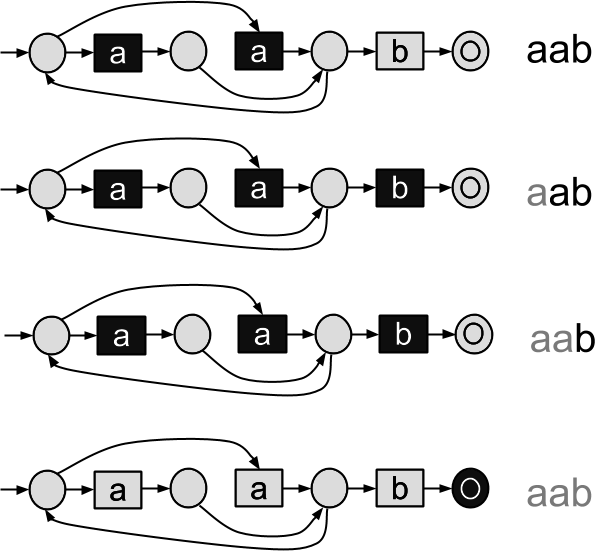
\includegraphics[scale=0.5]{figures/nfa_simultaneo.png}
  \caption{Passos do \emph{match} da expressão $(a|a)+b$ contra a entrada \emph{aab}}
  \label{fig:nfa_simultaneo}
\end{figure}

\emph{Vantagem}: Tem tempo de execução polinomial ($O(n \times m)$). Só precisa ler a entrada uma vez. Não requer uso de pilha.

\emph{Desvantagem}: Precisa de memória adicional para guardar os estados executados ($O(m)$). Em comparação com execução com DFA puro, é mais lento.

\subsection{Conversão preguiçosa para DFA}

O maior perigo da conversão completa para DFA é o potencial explosivo que a geração do autômato determinístico tem. Até $2^n$ estados podem ser gerados, e tempo proporcional a isso será gasto. Por outro lado, a simulação parelela parece gastar uma quantidade linear de memória e tempo polinomial para simular o autômato.

Para a maior parte dos autômatos reais, dificilmente a quantidade de estados no DFA será tão grande. Por isso, uma aproximação combinada entre as duas abordagens poderia trazer vantagens.

Durante a simulação paralela, os estados ativados simultaneamente correspondem exatamente a um estado no respectivo DFA. A realizar cache destes estados (porém mantendo uma política de gerência de memória, descartando os mais antigos) a implementação estará mantendo a complexidade de execução da simulação paralela, porém aumentando as chances de eventualmente gerar o DFA completamente.

\emph{Vantagem}: Tem tempo de execução linear no caso médio ($O(n)$). Só precisa ler a entrada uma vez. Não requer uso de pilha.

\emph{Desvantagem}: Pior caso ainda é $O(n \times m)$. Precisa de memória adicional para guardar os estados executados e o cache de estados do DFA. Implementação consideravelmente mais complexa.

%======================================================================================
\chapter{Implementação}
%======================================================================================

Neste capítulo será apresentada a implementação da biblioteca \emph{PyRex} (expressões regulares em Python). A implementação na íntegra pode ser visualizada no apêndice~\ref{app:full_source}.

\section{Considerações Iniciais}

Este projeto visava alcançar uma implementação completamente polinomial para expressões regulares. Alcançado o primeiro objetivo, o foco da implementação foi a simplicidade. Foram evitados truques de implementação que a tornassem mais rápida em detrimento da legibilidade. Todas as escolhas foram para reduzir a complexidade da implementação. Mesmo assim, o algoritmo utilizado foi eficiente o bastante para comprovar o ponto deste trabalho.

A linguagem escolhida para implementar o projeto foi Python. É uma linguagem de máquina virtual, tal qual o Java. Entretanto, sua máquina virtual não tem as otimizações em tempo de execução que as implementações mais famosas de Java tem. Além disso, sua resolução dinâmica de tipos a faz ter uma performance inferior a outra linguagens com resolução estática de tipos. 

Mesmo assim, pela reduzida quantidade de caracteres especiais em sua sintaxe, os programas escritos nela são em geral mais legíveis e simples. Por isso, toda a implementação do PyRex tem 85 linhas de código (contando as em branco) e cerca de 2.5KiB. Esta implementação abrange desde o parse da expressão regular até a simulação do autômato retornando inclusive a região do match da expressão regular.

O projeto foi implementado utilizando apenas as bibliotecas padrão disponíveis no Python 2.7, porém ele também funciona no Python 3.0 e superiores.

\section{Funcionalidades Implementadas}

Foi escolhido um conjunto de funcionalidades que fosse capaz de mostrar o ponto de falha das implementações modernas de expressões regulares e ainda assim ser simples o suficiente para ter uma implementação que pudesse ser explicada em alguns minutos.

Assim, foi implementado o match de:

\begin{lcircp}
    \item Literais (e.g. $a$)
    \item Sequências (e.g. $ab$)
    \item Alternâncias (e.g. $ab|cd$)
    \item Agrupamentos (e.g. $a(bc)d$)
    \item Expressão opcional (e.g. $a?$)
    \item Kleene* (e.g. $a*$)
    \item Kleene+ (e.g. $a+$)
\end{lcircp}

Estas funcionalidades são bem próximas as definidas por Thompson \cite{bib:Thompson68} em seu artigo e definem inequivocamente gramáticas regulares.

\section{Estrutura do Código}

O código está dividido em basicamente duas partes: um \emph{parser} e um \emph{matcher}.

O parser é responsável por receber uma string com a expressão regular, analisá-la sintaticamente e retornar um objeto (o matcher) capaz de reconhecer strings que façam parte da linguagem regular definida.

O matcher contém informações do autômato gerado e contém funções que sabem simular a execução do autômato. Ele é implementado como uma classe Python com um método \emph{match}, além da sobrecarga do operador \emph{\_\_repr\_\_} do Python, que provê uma visualização útil do objeto em tempo de debugging.

O parser é implementado pela função \emph{rex}. E o matcher pela classe \emph{Machine}.


\section{Análise sintática}

Análise sintática é feita pela função \emph{rex}. Ela implementa um parser recursivo descendente rudimentar. A BNF está descrita abaixo:

\begin{verbatim}
<option>     ::= <sequence> { "|" <sequence> }*
<sequence>   ::= { <repetition> }*
<repetition> ::= <primary> { "*" | "?" | "+" }*
<primary>    ::= "." | <literal> | "(" <option> ")"
\end{verbatim}

É importante chamar atenção ao detalhe da regra \emph{sequence} que permite strings vazias. Esta é uma mudança que permite strings vazias como expressão regular (o que é útil em alguns casos). Entretanto, esta mesma mudança permite expressões regulares do tipo $a||b$. O que não chega a constituir um erro. A listagem~\ref{lst:sequence} mostra a implementação desta regra.

\vspace{0.5cm}
\begin{lstlisting}[caption={Implementação da regra \emph{sequence}},label=lst:sequence]
def sequence():
    e = []
    while tokens and tokens[0] not in '|)':
        e += repetition()
    return e
\end{lstlisting}

A implementação é bastante simplista, usa uma instância da classe \emph{deque} como buffer de tokens e chamadas recursivas para implementar as regras. Para cada uma das quatro regras defindas pela BNF, há um método aninhado em \emph{rex} para representá-la.

O tratamento de erros é simples porém eficiente. Sempre que um caractere não esperado é encontrado na entrada, ele é reportado. Um dos mecanismos pode ser observado no código principal do parser (listagem~\ref{lst:main_parser}), onde após consumir todos os caracteres possíveis, se ainda existir remanescentes na entrada, uma exceção é lançada.

\vspace{0.5cm}
\begin{lstlisting}[caption={Implementação top-level do parser},label=lst:main_parser]
e = option()
if tokens: 
    raise Exception('Not expected: "{}"'.format(''.join(tokens)))

return Machine(e)
\end{lstlisting}

\section{Representação}

Durante o parse, a expressão regular é transformada numa representação do autômato relacionado. Este autômato é representado como um \emph{array de objetos}, onde cada posição do array representa um estado do autômato.

Como definido na seção~\ref{sec:Notacao} (página~\pageref{sec:Notacao}), a notação utilizada neste autômato prevê três tipos de estado: consumo, decisão e aceite. Estados de consumo são representados pelo caractere que consomem. Estados de decisão são representados por uma tupla de inteiros que informam quantos estados à frente ou atrás deve-se `pular'. Estados de aceite não precisam de representação, pois sempre ocorrem no final do autômato (segundo esta notação).

A figura~\ref{fig:exemplo_automato_puro} e as listagens \ref{lst:automaton_array} e \ref{lst:automaton_instr} representam a expressão regular $(a|a)+b$. Apenas a forma em array é armazenada na instância da classe Machine para execução. Entretanto, a forma em instruções pode ser gerada através do método \emph{\_\_repr\_\_} da mesma classe.

\begin{figure}[ht]
  \centering
  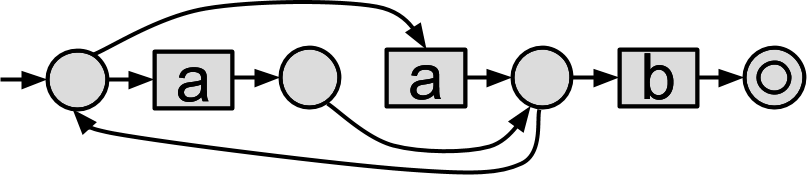
\includegraphics[scale=0.4]{figures/exemplo_automato_puro.png}
  \caption{Representação do autômato como diagrama de estados}
  \label{fig:exemplo_automato_puro}
\end{figure}


{
  \lstset{%
    basicstyle=\ttfamily\normalsize,
  }
  \begin{lstlisting}[caption={Representação do autômato como array},label=lst:automaton_array]
	[(1, 3), 'a', (2,), 'a', (1, -4), 'b']
  \end{lstlisting}
}

{
  \lstset{%
    basicstyle=\ttfamily\normalsize,
  }
  \begin{lstlisting}[caption={Representação do autômato como instruções},label=lst:automaton_instr]
0000: JUMP (1, 3)
0001: CONSUME a
0002: JUMP (2,)
0003: CONSUME a
0004: JUMP (1, -4)
0005: CONSUME b
0006: MATCH!
  \end{lstlisting}
}


\section{Simulação}

A simulação é executada pelos métodos \emph{matcher} e \emph{match} da classe \emph{Machine}. A diferença entre os dois é que o primeiro retorna um iterador que exibe o estado da execução do autômato para cada caractere da entrada. O segundo apenas retorna o resultado do match no final. Na implementação, o método \emph{match} utiliza o método \emph{matcher}, como mostra a listagem~\ref{lst:match}.

\vspace{0.5cm}
\begin{lstlisting}[caption={Implementação do método \emph{match}},label=lst:match]
def match(self, string):
    return reduce(lambda answer, s: s[0], self.matcher(string), None)
\end{lstlisting}

O método implementado para a simulação do autômato é a \emph{simulação paralela}. Este método foi escolhido por combinar uma complexidade assintótica polinomial com uma facilidade de implementação razoável.

A implementação baseia-se em duas listas, A e B, que em todo momento representam o conjunto de estados \emph{de consumo} alcançados até o início da avaliação do caractere atual (A) e o conjunto de estados que a avaliação do caractere atual irá alcançar (B). Após a avaliação de cada caractere estas listas são invertidas. É importante ressaltar que um mesmo estado nunca entra na lista B duas vezes. Esta verificação é efetuada pelo array V, que controla o índice do último caractere onde cada estado entrou na lista de estados. Inicialmente, esta lista está preenchida com valores -1.

Como apenas estados de consumo entram nas listas de estados para participar do ciclo de consumo (por razões óbvias), é preciso avaliar todos os estados de decisão antes do início do ciclo de consumo. A listagem \ref{lst:addnext} mostra a implementação do método \emph{addnext} que adiciona estados à próxima lista de consumo (B), resolvendo estados de decisão em seus respectivos próximos estados de consumo. Este método também retorna o número de vezes que o estado de aceite foi alcançado.

\vspace{0.5cm}
\begin{lstlisting}[caption={Implementação do método \emph{addnext}},label=lst:addnext]
def addnext(start, i, j):
    if j==self.n: return 1
    if V[j] == i: return 0
    V[j] = i

    if isinstance(self.states[j], tuple):
        return sum(addnext(start, i, j+k) for k in self.states[j])

    B.append((start, j))
    return 0
\end{lstlisting}

Cada ciclo de consumo é marcado por uma série de passos

Como é costumeiro na implementação de expressões regulares, o match é realizado caso qualquer substring do input faça match. O método de simulação paralela leva vantagem por necessitar de pouca alteração para suportar este modo de execução.



\section{Modo de uso}

TBD

\section{Visualização e Testes}

TBD


%======================================================================================
\chapter{Análise dos Resultados}
%======================================================================================

TBD

%======================================================================================
\chapter{Conclusão}
%======================================================================================

TBD

\backmatter

\appendix

\postextualchapter{Código-fonte da Biblioteca PyRex}\label{app:full_source}

\begin{lstlisting}[language=python]
from collections import deque
from functools import reduce

def rex(pattern):
    tokens = deque(pattern)

    def walk(chars):
        while tokens and tokens[0] in chars:
            yield tokens.popleft()

    def option():
        e = sequence()
        for token in walk('|'):
            e2 = sequence()
            e = [(1, len(e)+2)] + e + [(len(e2)+1,)] + e2
        return e        

    def sequence():
        e = []
        while tokens and tokens[0] not in '|)':
            e += repetition()
        return e
        
    def repetition():
        e = primary()
        for token in walk('?*+'):
            if token in '+*': e = e + [(1, -len(e))]
            if token in '?*': e = [(1, len(e)+1)] + e
        return e
        
    def primary():
        token = tokens.popleft()
        if token == '.': return [None]
        if token == '(': return [option(), tokens.popleft()][0]
        if token not in '?*+)|': return [token]
        raise Exception('Not expected: "{}"'.format(token))

    e = option()
    if tokens: 
        raise Exception('Not expected: "{}"'.format(''.join(tokens)))

    return Machine(e)
                
class Machine(object):
    def __init__(self, states):
        self.states = states
        
    def match(self, string):
        A, B, V = deque(), deque(), set()
             
        def best(a, b):
            if not a or not b: return a or b
            return a if a[0]<b[0] or a[0]==b[0] and a[1]>b[1] else b
                
        def addnext(start, i, j):
            if j==len(self.states): return (start, i)
            if j in V or V.add(j): return

            state = self.states[j]
            if isinstance(state, tuple):
                return reduce(best, (addnext(start, i, j+k) for k in state))
            else:
                B.append((start, j))
        
        def advance(i, c):
            while A:
                start, j = A.popleft()
                if self.states[j] in (None, c):
                    yield addnext(start, i+1, j+1)
        
        answer = None
        for i, c in enumerate(string):
            addnext(i, i, 0)
            A, B, V = B, A, set()
            answer = reduce(best, advance(i, c), answer)           

        return answer
       
    def source(self):
        for s in self.states:
            yield ('JUMP ' if isinstance(s, tuple) else 'CONSUME ') + str(s)
        yield 'MATCH!'
       
    def __repr__(self):
        return '\n'.join('{:04d}: {}'.format(i, s) for i, s in enumerate(self.source()))
\end{lstlisting}   

%======================================================================================
\postextualchapter{Benchmark em Python: re, pyrex}
%======================================================================================

\section{Tabela de Tempos (em microsegundos)}

\begin{center}
	\vline
	\begin{tabular}{ c || c | c }
		{\bf n} & {\bf re} & {\bf pyrex} \\
		\hline 
		1 & 5 & 20  \\ 
		2 & 4 & 23 \\ 
		3 & 3 & 27 \\ 
		4 & 3 & 33 \\ 
		5 & 3 & 39 \\ 
		6 & 4 & 44 \\ 
		7 & 6 & 50 \\ 
		8 & 6 & 55 \\ 
		9 & 9 & 61 \\ 
		10 & 13 & 67 \\ 
		11 & 22 & 73 \\ 
		12 & 33 & 79 \\ 
		13 & 55 & 91 \\ 
		14 & 84 & 95 \\ 
		15 & 133 & 100 \\ 
		16 & 221 & 103 \\ 
		17 & 353 & 108 \\ 
		18 & 566 & 114 \\ 
		19 & 927 & 121 \\ 
		20 & 1486 & 129 \\ 
	\end{tabular}
	\vline
	\quad
	\vline
	\begin{tabular}{ c || c | c }
		{\bf n} & {\bf re} & {\bf pyrex} \\
		\hline 
		21 & 2409 & 136 \\ 
		22 & 3875 & 142 \\ 
		23 & 6438 & 159 \\ 
		24 & 10251 & 153 \\ 
		25 & 17418 & 178 \\ 
		26 & 26590 & 177 \\ 
		27 & 42723 & 189 \\ 
		28 & 68890 & 190 \\ 
		29 & 111910 & 198 \\ 
		30 & 181338 & 201 \\ 
		31 & 296340 & 212 \\ 
		32 & 478507 & 219 \\ 
		33 & 763335 & 222 \\ 
		34 & 1259066 & 228 \\ 
		35 & 1937591 & 232 \\ 
		36 & 3136469 & 240 \\ 
		37 & 5078676 & 246 \\ 
		38 & 8261930 & 250 \\ 
		39 & 13229837 & 256 \\ 
		40 & 21334059 & 262 \\
	\end{tabular}
	\vline
\end{center}

\newpage
\section{Gráfico}

\begin{figure}[ht]
  \centering
  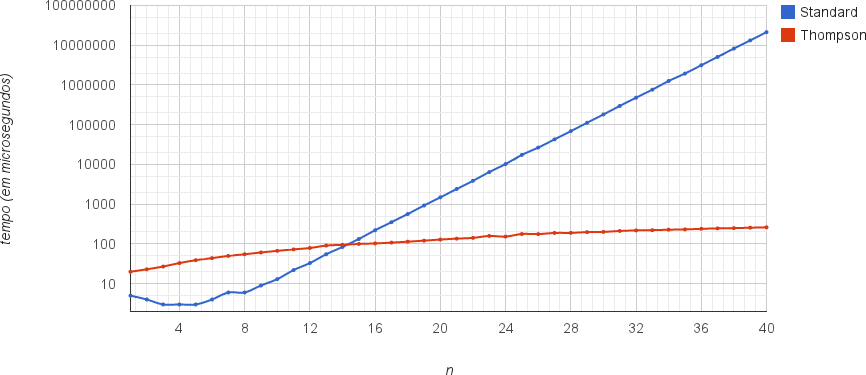
\includegraphics[scale=0.5]{figures/benchmark1.png}
\end{figure}

\section{Código fonte}

\begin{lstlisting}[language=python]
import re, pyrex

from timeit import timeit

r1 = re.compile('(a?a)+b')
r2 = pyrex.rex('(a?a)+b')

def time(r, i):
    return timeit(lambda: r.match('a'*i), number=1)*1e6

for i in xrange(1, 41):
    print '{}\t{:8.0f}\t{:8.0f}'.format(
        i, time(r1, i), time(r2, i))
\end{lstlisting}

     
   

\bibliography{bibliografia}

\end{document}

